\documentclass[tikz,border=8pt]{standalone}
\usepackage{amsmath}
\begin{document}
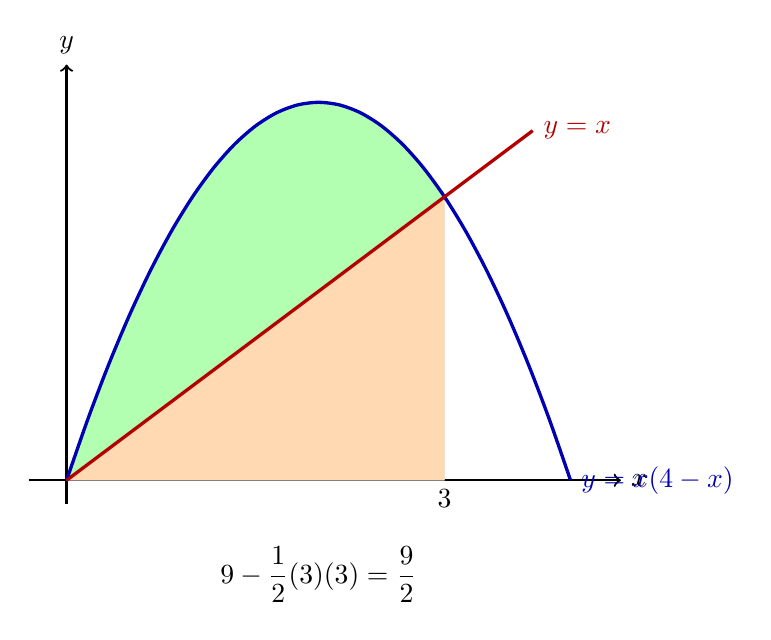
\begin{tikzpicture}[xscale=1.6,yscale=1.2]
\draw[->,thick] (-0.3,0)--(4.4,0) node[right] {$x$};
\draw[->,thick] (0,-0.25)--(0,4.4) node[above] {$y$};
\fill[blue!15] (0,0)--plot[smooth,domain=0:3] (\x,{\x*(4-\x)})--(3,0)--cycle;
\fill[orange!30] (0,0)--(3,3)--(3,0)--cycle;
\fill[green!30] (0,0)--plot[smooth,domain=0:3] (\x,{\x*(4-\x)})--(3,3)--cycle;
\draw[very thick,blue!70!black] plot[smooth,domain=0:4] (\x,{\x*(4-\x)}) node[right] {$y=x(4-x)$};
\draw[very thick,red!70!black] (0,0)--(3.7,3.7) node[right] {$y=x$};
\node[below] at (3,0) {$3$};
\node at (2,-1) {$\displaystyle 9-\frac12(3)(3)=\frac92$};
\end{tikzpicture}
\end{document}